\documentclass[a4paper,10pt]{article}
\usepackage[utf8]{inputenc}

\usepackage{framed}
\usepackage{algorithm}
\usepackage{algpseudocode}


\usepackage{amsthm}
\usepackage{amsmath}
\usepackage{amssymb}
\usepackage{changebar}

\title{Milestones in solving games on graphs}
\author{Sasha Rubin}
\date{\today}

\newcommand{\pz}{Player $0$\xspace}
\newcommand{\po}{Player $1$\xspace}

%% PACKAGES %%
\usepackage{latexsym}
\usepackage{amsmath}
\usepackage{amssymb}
%\usepackage{amsthm} %


\usepackage{color}
\usepackage{graphicx}
\usepackage{tikz,pgf}
  \usetikzlibrary{automata,positioning,matrix,calc,petri,arrows}

%% ENVIRONMENTS %%
%\theoremstyle{plain}
%\newtheorem{theorem}{Theorem}
%\newtheorem{lemma}{Lemma}
%\newtheorem{fact}{Fact}
%\newtheorem{example}{Example}
%\newtheorem{definition}{Definition}
%%\newtheorem{corollary}{Corollary}
%\newtheorem{proposition}{Proposition}
%%\newtheorem*{proof*}{Proof}

%% COMMENTS %%

\newcommand\note[1]{{\color{red}{#1}}}
\newcommand{\todo}[1]{{{\color{blue} #1}}}
%\renewcommand{\todo}[1]{}

%% LATEX SHORTCUTS %%
% cause problems with aamas style file
%\def\it{\begin{itemize} }
%\def\-{\item[-] }
%\def\ti{\end{itemize} }
%\def\en{\begin{enumerate} }
%\def\ne{\end{enumerate} }

%% COMPLEXITY CLASSES %%

\def\UPTime{\textsc{up}\xspace}
\def\CoUPTime{\textsc{coup}\xspace}


\def\exptime{\textsc{exptime}\xspace}
\def\exptimeC{\exptime-complete}

\def\pspace{\textsc{pspace}\xspace}
\def\pspaceC{\pspace-complete}

\def\logspace{\textsc{logspace}\xspace}
\def\nlogspace{\textsc{nlogspace}\xspace}

\def\ptime{\textsc{ptime}}
\def\np{\textsc{np}}



%% LOGIC %%
\def\fol{\mathsf{FOL}}
\def\SL{\textsf{SL}}

\def\msol{\mathsf{MSOL}}
\def\fotc{\mathsf{FOL+TC}}

\def\know{\mathbb{K}}
\def\dknow{\mathbb{D}}
\def\cknow{\mathbb{C}}
\def\eknow{\mathbb{E}}

\def\dualknow{\widetilde{\mathbb{K}}}
\def\dualdknow{\widetilde{\mathbb{D}}}
\def\dualcknow{\widetilde{\mathbb{C}}}
\def\dualeknow{\widetilde{\mathbb{E}}}

\renewcommand\implies{\rightarrow}

%% TEMPORAL LOGIC %%
\newcommand{\sqsq}[1]{\ensuremath{[\negthinspace[#1]\negthinspace]}}

\DeclareMathOperator{\ctlE}{{\mathsf{E}}}
\DeclareMathOperator{\ctlA}{\mathsf{A}}


\newcommand{\atlE}[1][A]{\ensuremath{\langle\!\langle{#1}\rangle\!\rangle}}
\newcommand{\atlA}[1][A]{\ensuremath{[[{#1}]]}}

\DeclareMathOperator{\nextX}{\mathsf{X}}
\DeclareMathOperator{\yesterday}{\mathsf{Y}}
\DeclareMathOperator{\until}{\mathbin{\mathsf{U}}}
\DeclareMathOperator{\weakuntil}{\mathbin{\mathsf{W}}}
\DeclareMathOperator{\since}{\mathbin{\mathsf{S}}}
\DeclareMathOperator{\releases}{\mathbin{\mathsf{R}}}
\DeclareMathOperator{\always}{\mathsf{G}}
\DeclareMathOperator{\hitherto}{\mathsf{H}}
\DeclareMathOperator{\eventually}{\ensuremath{\mathsf{F}}\xspace}
\DeclareMathOperator{\previously}{\mathsf{P}}
\newcommand{\true}{\mathsf{true}}
\newcommand{\false}{\mathsf{false}}


\newcommand{\LTL}{\ensuremath{\mathsf{LTL}}\xspace}
\newcommand{\PLTL}{\textsf{PROMPT-}\LTL}

\newcommand{\CTL}{\ensuremath{\mathsf{CTL}}\xspace}
\newcommand{\CTLS}{\ensuremath{\mathsf{CTL}^*}\xspace}
\newcommand{\PCTLS}{\textsf{PROMPT-}\CTLS}
\newcommand{\PCTL}{\textsf{PROMPT-}\CTL}
\newcommand{\CLTL}{\ensuremath{\textsf{C-}\LTL}\xspace}
\newcommand{\PCLTL}{\ensuremath{\textsf{PROMPT-C}\LTL}\xspace}

\newcommand{\ATL}{\ensuremath{\mathsf{ATL}}\xspace}
\newcommand{\ATLS}{\ensuremath{\mathsf{ATL}^*}\xspace}
\newcommand{\PATLS}{\textsf{PROMPT-}\ATLS}
\newcommand{\PATL}{\textsf{PROMPT-}\ATL}

\newcommand{\KATL}{\ensuremath{\mathsf{KATL}}\xspace}
\newcommand{\KATLS}{\ensuremath{\mathsf{KATL}^*}\xspace}
\newcommand{\PKATLS}{\textsf{PROMPT-}\KATLS}
\newcommand{\PKATL}{\textsf{PROMPT-}\KATL}


\def\red{{red}}
\def\col{{col}}
\def\alt{\, | \,}

%% PROMPT 
\def\kmodels{\models^k}
\def\twokmodels{\models^{2k}}
\DeclareMathOperator{\Fp}{\eventually_\mathsf{P}}
\DeclareMathOperator{\Gp}{\always_\mathsf{P}}
\DeclareMathOperator{\within}{\mathsf{within}}

\newcommand{\AP}{{AP}}
\def\Ag{{Ag}}
\def\Act{{Act}}

%% MATH OPERATIONS %%
\newcommand{\tpl}[1]{\langle {#1} \rangle }
\newcommand{\tup}[1]{\overline{#1}}
\def\proj{\mathsf{proj}}
\newcommand{\defeq}{\ensuremath{\triangleq}}

%% STRUCTURES and STRATEGIES %%
\newcommand{\cgs}{\ensuremath{\mathsf{S}}}
\newcommand{\LTS}{\mathsf{S}}
\newcommand{\Comp}{\mathsf{cmp}}
\newcommand{\Hist}{\mathsf{hist}}
\newcommand{\out}{{out}}

\newcommand{\Paths}{\mathsf{pth}}

\newcommand{\nat}{\mathbb{N}}
\def\int{\mathbb{Z}}
\newcommand{\natzero}{\mathbb{N}_0}

\newcommand{\trans}[3]{#1 \stackrel{\mathsf{#3}}{\rightarrow} #2}


%% HEADINGS ETC %%
\newcommand{\head}[1]{\noindent {\bf #1}.}

%% COUNTER MACHINES %%
\newcommand{\cm}{M}
\newcommand{\CMinc}{\mathsf{inc}}
\newcommand{\CMdec}{\mathsf{dec}}
\newcommand{\CMzero}{\mathsf{ifzero}}
\newcommand{\CMnonzero}{\mathsf{nzero}}
\newcommand{\CMcommit}{\mathsf{end}}


%% CLTL %%
\def\var{{\sf var}}
\def\ovar{{\sf ovar}}
\def\avar{{\sf avar}}
\def\svar{{\sf svar}}
\def\bvar{{\sf bvar}}

\def\MOD{\equiv}

%% PVP %%
\def\PVP{\mathsf{PVP}}



\newcommand{\q}{\textbf{Question:} }
\newcommand{\reach}[1]{\textsc{Reach}(#1)}
\newcommand{\rep}[1]{\textsc{B\"uchi}(#1)}

\newcommand{\safe}[1]{\textsc{Safe}(#1)}

\newcommand{\obj}{Obj}
\newcommand{\cpre}{\textrm{CPre}}
\newcommand{\rank}{\textrm{rank}}
\newcommand{\WR}{\textrm{WR}}
\newcommand{\att}{\textrm{Att}}

\begin{document}

\maketitle


\section{Outline}

Games on graphs are a useful mathematical model of many phenomena in
computer science that involve interaction between
players/agents/components.  Solving a game means deciding if a given
player has a winning strategy. There are a number of classes of games
whose complexity are in $NP \cap coNP$, but are not known to be in P,
i.e., parity games, mean-payoff games, discounted payoff games, simple
stochastic games. This year, there was a breakthrough in the analysis
of parity games, a deceptively simply class of games with tight
connections to deep results in logic and automata theory. A team from
New Zealand and Singapore [Calude et. al. 2017] gave a
quasi-polynomial time algorithm for solving parity games --- previous
algorithms were mildly subexponential.  We will chart a course through
the theory of games on graphs, studying determinacy, memory required
for winning, and the complexity of solving games. We will start with
foundational work and end with very recent results.

Participants will give a talk on a classic or current paper. There are
a variety of topics to choose from: the tight connection between
graph-games and logic and automata-theory, the use of graph-games in
formal-methods (modeling, verification, synthesis, testing,
composition, simulation), the use of graph-games in AI (automated
planning, verification in robotics, general-game playing), or
extensions of the basic model (multiplayer games, partial-information
games, stochastic games, pushdown games, timed games).


\subsection{Core Papers}
\begin{itemize} 
 \- Ehrenfeucht and Mycielski (1979). Positional strategies for mean
  payoff games.
\- McNaughton (1993). Infinite games played on finite graphs.

\- Zwick and Paterson (1995). The complexity of mean payoff games.
\- Dziembowski, Jurdzinski, and Walukiewicz (1997). How much memory is
  needed to win infinite games?
\- Zielonka (1998). Infinite games on finitely coloured graphs with
  applications to automata on infinite trees.
\- Voge and Jurdzinski (2000). A discrete strategy improvement
  algorithm for solving parity games.
\- Chatterjee, Henzinger, and Jurdzinski (2005). Mean-payoff parity
  games.
\- Schewe (2007). Solving Parity Games in Big Steps.
\- Jurdzinski, Paterson, and Zwick (2008). A deterministic
  subexponential algorithm for solving parity games.
\- Friedmann (2009). An exponential lower bound for the parity game
  strategy improvement algorithm as we know it.
\- Benerecetti, Dell'Erba and Mogavero (2016). Solving parity games via
  priority promotion.
\- Aminof and Rubin (2016). First Cycle Games.
\- Calude, Jain, Khoussainov, Li, and Stephan (2017). Deciding parity
  games in quasipolynomial time.
\- Jurdzinski and Lazic (2017). Succinct progress measures for solving
  parity games.
\end{itemize}

\subsection{Additional reading}
\it
\- Gradel, Thomas, and Wilke (Eds.) (2002). Automata, Logics, and
  Infinite Games: A Guide to Current Research.
\- Apt and Gradel (Eds.) (2011). Lectures in Game Theory for Computer
  Scientists.
\ti

\section{Where do games come from?} 

1. Where do games arise? Why analyse games?

2. Simple llustration of connection with logic.

\paragraph{Outline}
Games on graphs are a useful mathematical model of many phenomena in mathematics and computer science that involve interaction of two or more players. We will define games on graphs and mention a few scenarios where they arise, including automated planning in Artificial Intelligence, automata theory and mathematical logic.
We will illustrate by showing how one can think of evaluating Boolean formulas as a game on the parse tree of the formula.

\paragraph{Main idea: games capture strategic interactions.}

\paragraph{Model: two players moving a token along the edges of a graph, resulting in an infinite path called a play. \pz is trying to ensure 
the play is in a given set, and \po is trying to ensure it is outside the given set.}

\begin{definition}[Graphs, Arenas, Games]
\

\en
\- A \emph{graph} is a structure $(V,E)$ where $V$ is a set of vertices and $E \subseteq V \times V$ a set of edges.
\- An \emph{arena} is a structure $A = (V,E,V_0,V_1)$ in which $E$ is total, i.e., for every $v \in V$ there exists $w \in V$ such that $E(v,w)$ (we also say ``no dead-ends'').
\- A \emph{play} is an infinite path in $A$.
\- A \emph{game} is a structure $G=(A,\obj)$ where $\obj \subseteq V^\omega$ is an objective.
\ne
\end{definition}

In reachability games, \pz is trying to force a visit to $T$, and \po is 
trying to ensure the play never visits $T$.

\begin{definition}[Reachability]
 Let $T \subseteq V$ and define objective $\reach{T}$ to consist of all  $\pi$ such that some $\pi_i \in T$. In this case we say that $\pi$ \emph{reaches} $T$; otherwise $\pi$ \emph{avoids} $T$.
\end{definition}

\begin{center}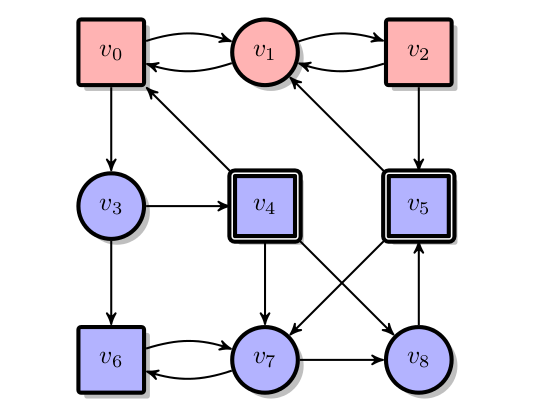
\includegraphics[width=6cm,height=4.6cm]{arena.png} \end{center}

\begin{example}
Calculate from which vertices player \po (round nodes) can force a visit to $T$ (the double-framed vertices)? \textbf{Draw} positional strategy.
\end{example}

\subsection{Why play games?}

\begin{center}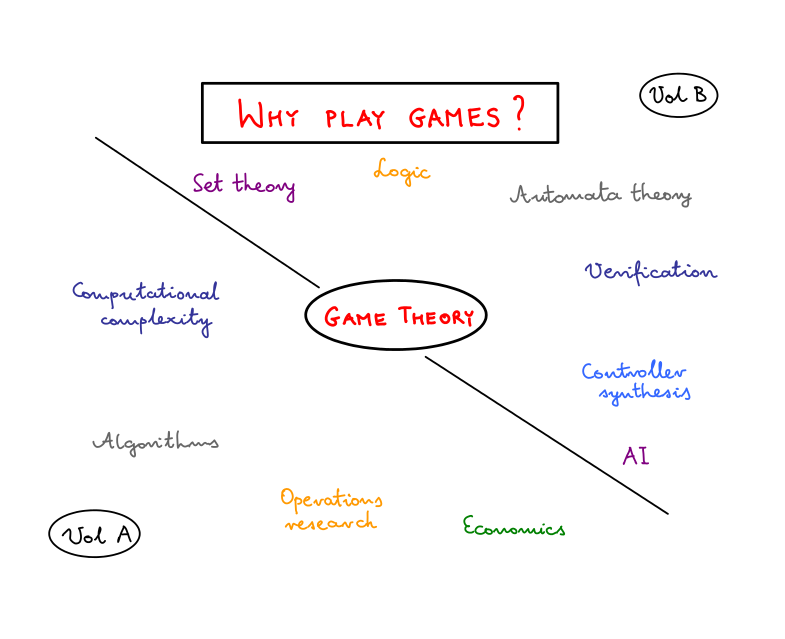
\includegraphics[width=7cm,height=7cm]{whyplay.png} \end{center}


\paragraph{Motivations/applications}

\it
\- Games in logic: evaluating logic formulas
\- Games humans play: the game-tree is a graph-game.
\- Games from algorithms: graph reachability to sabotage games
\- Games in automata: gives semantics to alternating automata 
\- Games in verification/AI: games model reactive systems, strategies model controllers.
\- Economics/Game theory: mathematical theory of how agents, e.g., people, 
behave in strategic scenarios; games in extensive form; graphical games.
\- Games in set theory: determinacy in games used to prove that one can 
reverse quantifiers in mathematical statements.
\- Computational complexity: alternating TM/time/space.
\ti



\paragraph{Games humans play}

\begin{question}
 How can you think of games humans play as games on graphs?
\end{question}

\en
\- Vertices correspond to ``snapshots'' called \emph{configurations}.
\- Edges correspond to one-step moves in the game. Get a tree or a DAG.
\- Objectives correspond to the winning plays. E.g., $Obj$ is the set of plays such that the first player to make a row of three is player 0.
\ne

To make this a reachability game, you should loop the first time someone wins and then let $T$ be the set of winning configurations.

If a game has finitely many rounds, then $T$ is finite. In this case, 
we can solve the game in $\logspace$ in the size of $T$. How?

Is this useful?

% N.B. The size of $T$, in this case, is often exponentially more succinct than the description of the game.

\it 
\- tic-tac-toe (\emph{tris}) has $9!$ vertices in the game-tree (approx $10^5$).
\- chess (\emph{scacchi}) has at least $10^{120}$ vertices in the game-tree (Shannon, 1950), and about $10^{40}$ positions in game-graph.
\ti

% CHESS! Game tree = 
% vertices are snapshots of board, edges are one step moves, turn depends on 
% depth (even/odd), white goes first, assume rule for draw ends the game, leaf is 
% marked with a $1$ if white checkmates black, and $0$ otherwise (draw or lose). 
% Give estimate of size of game-tree. 

% It is easy to see that white has a winning strategy in chess iff \pz $A$ has a strategy in the game-tree 
% that forces the play to visit $T$. So, does white have a winning strategy? Why is this a hard problem? 


\paragraph{Controller synthesis}
An open/reactive system is one with controllable and uncontrollable events. This can be thought of as a game between a controller/system player 
and an environment player. Controllers are strategies that say how to control the variables.

\begin{question}
 What are the controllable events,  uncontrollable events, and objectives in the following open systems: ATM machines, Anti-lock braking system in car.
\end{question}

 \en
 \- ATM machine: controllable = internal state of the system, uncontrollable = what actions people will do using the ATM, objective = always give correct amount of money, ensure security, etc.

 \- Anti-lock braking system in car: controllable = how much to apply breaks to each wheel, uncontrollable = 
sensor readings like the speed of each wheel, objective = maintain uniform wheel speed.
 \ne

 \paragraph{Positional strategies}
\begin{definition}
Fix a game $G = (V,V_0,V_1,E,\obj)$. 
\it
\- A \emph{positional strategy} for player $i$ is a 
function $\sigma:V_i \to V$ such that $(v,\sigma(v)) \in E$. 
\- A play $\rho = \rho_0 \rho_1 \dots$ is consistent with $\sigma$ if 
whenever $\rho_j \in V_i$, $\rho_{j+1} = \sigma(\rho_j)$.
% % \- If $\sigma_i$ is a strategy for player $i$ and $v \in V$ then 
% % $play_v(\sigma_0,\sigma_1)$ is the unique sequence $\rho = \rho_0 
% % \rho_1 \dots$ such that $\rho_0 = v$ and if $\rho_k \in V_i$ then 
% % $\rho_{k+1} = \sigma_i(\rho_k)$. 
% \- A strategy $\sigma_0$ is \emph{winning} if for 
% all strategies $\sigma_1$ of player $1$, $play_v(\sigma_0,\sigma_1) \in \obj$.
\- A strategy $\sigma_0$ for player $0$ is \emph{winning} if for all plays $\rho$ consistent with 
$\sigma_0$, we have that $\rho \in \obj$. A strategy $\sigma_1$ for player $1$ is winning 
if for all plays $\rho$ consistent with $\sigma_1$, we have that $\rho \not \in \obj$.
\ti
\end{definition}


\paragraph{Example. Games for evaluating formulas}

\begin{example}
We consider propositional formulas without negation. e.g., 
\[ ((a \wedge b) \vee c) \vee (a \wedge c) \] and valuation $v:a \mapsto 1, b \mapsto 1, c \mapsto 0$.
\end{example}

\begin{question}
\en
\- How does one evaluate the formula? Label parse tree bottom up.
\- How does one evaluate it top down? \textbf{Draw} winning strategy for \po.
\ne
\end{question}
 




\begin{definition}
Let $\Phi$ be a positive Boolean formula, and $v$ a valuation of its variables.
 The \emph{evaluation game} of $\phi,v$ is the reachability game 
 \[ 
G_{\phi,v} = (V,V_0,V_1,E,\reach{T})  
 \]
where 
\it
\- $V$ is the set of subformulas of $\phi$, 
\- $V_0 \subseteq V$ are those subformula whose 
top operation is $\vee$, 
\- $V_1$ are the rest, 
\- $T$ are those variables $x$ of $\phi$ such that $v(x) = 1$, and 
\- $E$ has transitions from $\varphi_1 \,  op \, \varphi_2$ to both $\varphi_1$ and to 
$\varphi_2$ for $op \in \{\wedge,\vee\}$, and from atoms to themselves.
\ti
\end{definition}

\begin{theorem}
Let $\Phi$ be a positive Boolean formula, and $v$ a valuation of its variables.
Then $v(\phi) = 1$ iff player $0$ has a winning strategy in 
$G_{\phi,v}$.
\end{theorem}

\begin{proof}
Induction on the formula. 

The base case is easy.

Consider the case that $\phi = \phi_1 \vee \phi_2$ (the case $\wedge$ is similar). Then TFAE:
\en
\- $v(\phi) = 1$ 
\- there exists $i$ such that $v$ satisfies $\phi_i$ 
\- there exists $i$ such such that \pz has a winning strategy in $G_{v,\phi_i}$ 
\- \pz has a winning strategy in $G_{v,\phi}$.
\ne

\begin{question}
 Prove that 3 implies 4.
\end{question}

We prove 3 implies 4: Let $\sigma$ be a winning strategy in $G_{v,\varphi_i}$. Define a strategy $\sigma'$ in $G_{v,\varphi}$ that first goes from the vertex $\varphi$ to $\varphi_i$, and then does $\sigma$. To see that $\sigma'$ is winning, let $\pi$ be a play in $G_{v,\varphi}$. Then the suffix of $\pi$ formed by removing the first vertex is a play in $G_{v,\phi_i}$. By assumption this suffix reaches $T$.

We prove 4 implies 3: Let $\sigma$ be a winning strategy in $G_{v,\varphi_1 \vee \varphi_2}$ and suppose 
$\sigma(\varphi_1 \vee \varphi_2) = \varphi_1$ (the case $\varphi_2$ is 
symmetric). 
Define a strategy $\sigma'$ on $G_{v,\varphi_1}$ to be the restriction of $\sigma$ to the 
subformulas of $\varphi_1$.
Let $\pi$ be a play in $G_{v,\varphi_1}$ consistent with $\sigma'$. We need to 
show it reaches $T$. But the play starting with $\varphi_1 \vee \varphi_2$ and 
then proceeding like $\pi$ is a play of $G_{v, \varphi_1 \vee \varphi_2}$ 
consistent with $\sigma$, and thus by assumption reaches $T$. Thus $\pi$ 
reaches $T$.
\end{proof}



% \- Corollary: deciding if player $E$ has a winning strategy is in ptime.


\begin{question} What is the game corresponding to evaluating arbitrary proposition 
formulas, i.e., allowing negation as an operator? 
\end{question}

% \- Homework: What properties of pairs of games captures logical equivalence?
% e.g., $p \wedge (q \vee r) \iff (p \wedge q) \vee (p \wedge r)$. In what sense 
% are these two games the same?


\section{Games with qualitative objectives} 
\paragraph{Outline} Games with qualitative objectives assign a winner to every play, e.g., reachability games. We will show how to solve reachability games. We will discuss how to compute winning strategies, and raise the issue of determinacy, and show how to solve games with more complex but still qualitative objectives.

\begin{definition}
% \- \emph{Arena} $A = (V,V_0,V_1,E)$, partition, directed, no 
% dead-ends. 
% % \- \emph{Subarena} $A' = (V', V_0 \cap V', V_1 \cap V', E \cap V' 
% % \times V')$... defined only if $E \cap V' \times V'$ has no deadends.
% \- \emph{Play}: $\rho = \rho_0 \rho_1 \cdots$ such that $(\rho_i,\rho_{i+1}) \in E$.
A \emph{strategy} for player $i$ is a function from $\sigma_i:V^*V_i \to V$ such 
that for $u \in V^*V_i$ we have that $(last(u),\sigma(u)) \in E$. 
Strategies $\sigma_0, \sigma_1$ induce a unique play, denoted $play_v(\sigma_0,\sigma_1)$.
A strategy $\sigma_0$ is \emph{winning from $v$} if for all strategies $\sigma_1$, the play $play_v(\sigma_0,\sigma_1) \in \obj$.
Call a play $\pi$ \emph{consistent} with strategy $\sigma_0$ if for every $u \in V^*V_i$ that is a prefix of $\pi$ we have that 
 $u \cdot \sigma_0(u)$ is a prefix of $\pi$. 
\end{definition}


\begin{question} 
 Prove that $\sigma_0$ is a winning strategy (i.e., beats all counterstrategies) iff every play $\pi$ consistent with $\sigma_0$ is in $\obj$.
\end{question}

\begin{definition}
The \emph{winning region} $W_i(G)$ of player $i$ is the set of vertices $v$ such that there exists a winning strategy $\sigma_i$ from $v$. 
\end{definition}

\begin{question}
Can a vertex be in both winning regions? Is every vertex in a winning region of one of the players? (come back to this later).
\end{question}


\begin{definition}
\emph{Solving a game} means computing the winning regions of both players, i.e., given G and $v$ and player $i$, decide if $v \in 
W_i(G)$.
\end{definition}


\begin{theorem}
 Solving reachability games is in \ptime. 
\end{theorem}

\begin{proof}
Fix a reachability game $G = (A,\reach{T})$ and $i = 0,1$. For $X \subseteq V$, define 
\begin{align*}
\cpre_i(X) & =  \{v \in V_i : \exists w \in X. (v,w) \in E\} \, \bigcup \\
&
\{v \in V_{1-i} : \forall w. (v,w) \in E \to w \in X\}
\end{align*}
and 
\begin{align*}
\att_i^0(X) &= X\\ 
\att_i^{k+1}(X) &= \att_i^k(X) \cup \cpre_i(\att_i^k(X)) \mbox{ for } k > 0.\\
\att_i(X) &=\cup_{k \geq 0} \att_i^k.
\end{align*}



\begin{question}
 Compute $\att_i(T)$ in the example. 
\end{question}

\begin{question} 
 Write the meaning of $\cpre_i(X)$, $\att_i^k(X)$ and $\att_i(X)$ in words.
 \it
 \- $v \in \cpre_i(X)$ iff player $i$ can force the play from $v$, in one step, to visit $X$.
 \- $v \in \att_i^k(X)$ iff player $i$ can force the play, in at most $k$ steps, to visit $X$. 
 \- $v \in \att_i(X)$ iff player $i$ can force the play to visit $X$. 
 \ti
\end{question}

\begin{question}
 Prove that $\att_i(T)$ is the least fix-point of the operation $X \mapsto T \cup \cpre_i(X)$.
\end{question}

We now prove that $\WR_i(G) = \att_i(T)$.  Let $\rank(v)$ be the smallest integer $k$ such that $v \in \att_i^k(T)$, and $\infty$ if there is no such $k$.

\paragraph{We prove that $\att_i(T) \subseteq \WR_i(G)$.}

Note the following:
\en
\- $v \in \att_i^k(T)$ implies $\rank(v) \leq k$.
\- $\rank(v) = 0$ iff $v \in T$.
\- If $v \in V_i \cap \att_i(T)$ and $0 < \rank(v)$ then some $(v,w) \in E$ has $\rank(w) < \rank(v)$.
\- If $v \in V_{1-i} \cap \att_i(T)$ and $0 < \rank(v)$ then every $(v,w) \in E$ has $\rank(w) < \rank(v)$.
\ne
Define a positional strategy $\sigma_i$ for player $i$ as follows: $\infty > \rank(v) > 0$ then define $\sigma_i(v)$ to be any vertex $v'$ with $\rank(v') < \rank(v)$, 
and otherwise define it arbitrarily.
Then $\sigma_i$ is winning from every $v \in \att_i(T)$: every play $\pi$ consistent with $\sigma_i$ starting at $v$, visits $T$ within $\rank(v)$-many steps. Proof is by induction on $\rank(v)$. If $\rank(v) = 0$ we are done. Suppose $ \rank(v) > 0$ and take $\pi$. The suffix of $\pi$ after one step is consistent with $\sigma$, and $\rank(\pi_1) < k$. By induction, this suffix visits $T$ within $k-1$ steps, and thus $\pi$ visits $T$ within $k$ steps.

\paragraph{We prove that $\WR_i(G) \subseteq \att_i(T)$.}

To see this it is sufficient to prove that $V \setminus \att_i(T) \subseteq \WR_{1-i}(G)$ (by ``squeezing'').


Note the following:
\en
\- If $v \in V_0$ and $\rank(v) = \infty$ then every $(v,w) \in E$ has $\rank(w) = \infty$.
\- If $v \in V_1$ and $\rank(v) = \infty$ then some $(v,w) \in E$ has $\rank(w) = \infty$.
\ne

Define a positional strategy $\sigma_{1-i}$ for Player $1-i$ as follows: for $v \in V_{1-i}$, if $\rank(v) = \infty$ then it maps $v$ to some $w$ with $(v,w) \in E$ and $\rank(w) = \infty$, and otherwise it is defined arbitrarily. Then $\sigma_{1-i}$ is winning from every $v$ with $\rank(v) = \infty$. Indeed, let $\pi$ be a play consistent with $\sigma_{1-i}$ starting with $v$ where $\rank(v) = \infty$. It is easy to see that $\rank(\pi_j) = \infty$ for all $j$ (formally, use induction on $j$). But $\rank(v) = 0$ for $v \in T$. Thus $\pi$ avoids $T$, so Player $1-i$ wins the play. 
\end{proof}

We have shown more. 

\begin{corollary} 
For reachability games:
\en
\- Player $i$ has a positional strategy that is winning from all vertices in $W_i(G)$, i.e., a \emph{uniform} winning strategy.
\- The winning regions partition $V$. This is called \emph{determinacy}.
\- The positional-winning regions partition $V$. This is called \emph{positional determinacy}.
\- The complexity of the algorithm is $O(|V||E|)$ (prove it can be done in $O(|E|)$).
\ne 
\end{corollary}

% \it
% \- Corollary: reachability games are determined, i.e., every vertex is in one 
% of the player's winning region. 
% \- Corollary: reach games are memoryless determined, i.e., $W_i(G) = MW_i(G)$.
% \- Determinacy, positionally determined
% \- Uniform position winning strategy: winning from every vertex in the winning 
% region



\begin{question}
Show how to solve the game in which player $0$ must, in at least one step, reach $T$, i.e., the objective consists of all sequence $\pi = \pi_0 \pi_1 \dots$ 
such that there exists $\pi > 0$ such that $\pi_i \in T$. Write $\att^+_0(X)$ for the attractor strategy.
\end{question}


\begin{question}
A safety game is one in which a player should not leave a set, i.e., $\safe{S}$ consists of all sequences $\pi$ such that $\pi_i \in S$ for all $i$. 
Show how to solve safety games, and that they are positionally determined. 
\end{question}




\begin{question}
Let $r$ be a regular expression over the vertices $V$ of an arena $A$. Define the objective $Obj_r$ to be 
the set of plays of $A$ for which some prefix matches $r$.

Show how to solve such games...

\en
\- convert $r$ into a DFW $M = (Q,\iota,\delta,F)$ (it is important the automaton is deterministic, why?)
\- form the product arena $A\times R$, i.e., vertices $V \times Q$, edges $(v,q)$ to $(v',q')$ if $E(v,v')$ and $\delta(q,v) = q'$.
\- player $i$'s vertices are $V_i \times Q$.
\- new objective $Obj_M$ is all sequences $(v_0,q_0) (v_1,q_1) ...$ such that $q_n \in F$ for some $n$.
\ne

Claim: player $0$ has a winning strategy in $(A,Obj_r)$ from $v$ iff player $0$ has a winning strategy in $(A \times R, Obj_M)$ from $(v,iota)$.

Moreover: ``strategies transfer'', and thus $(A,Obj_r)$ is positionally determined.

What is the complexity? (I guess EXPTIME-complete... upper bound is easy (subset construction); lower-bound?)


\end{question}

\subsection{Repeated reachability}

\begin{definition}
A set $X \subseteq V$ is a \emph{trap for player $i$} if player $1-i$ has a strategy $\sigma$ 
such that every play consistent with $\sigma$ starting in $X$ stays in $X$.
\end{definition}

Note that $V \setminus Att_i(T)$ is a trap for player $i$.

\begin{lemma}
 If $X$ is a trap then the graph restricted to vertices in $X$ is an arena (i.e., total).
\end{lemma}




\begin{definition}
The objective of a repeated-reachability game, $\rep{T}$, consists of all sequence $\pi$ such that infinitely many $i$ have $\pi_i \in T$. 
\end{definition}

% \begin{center}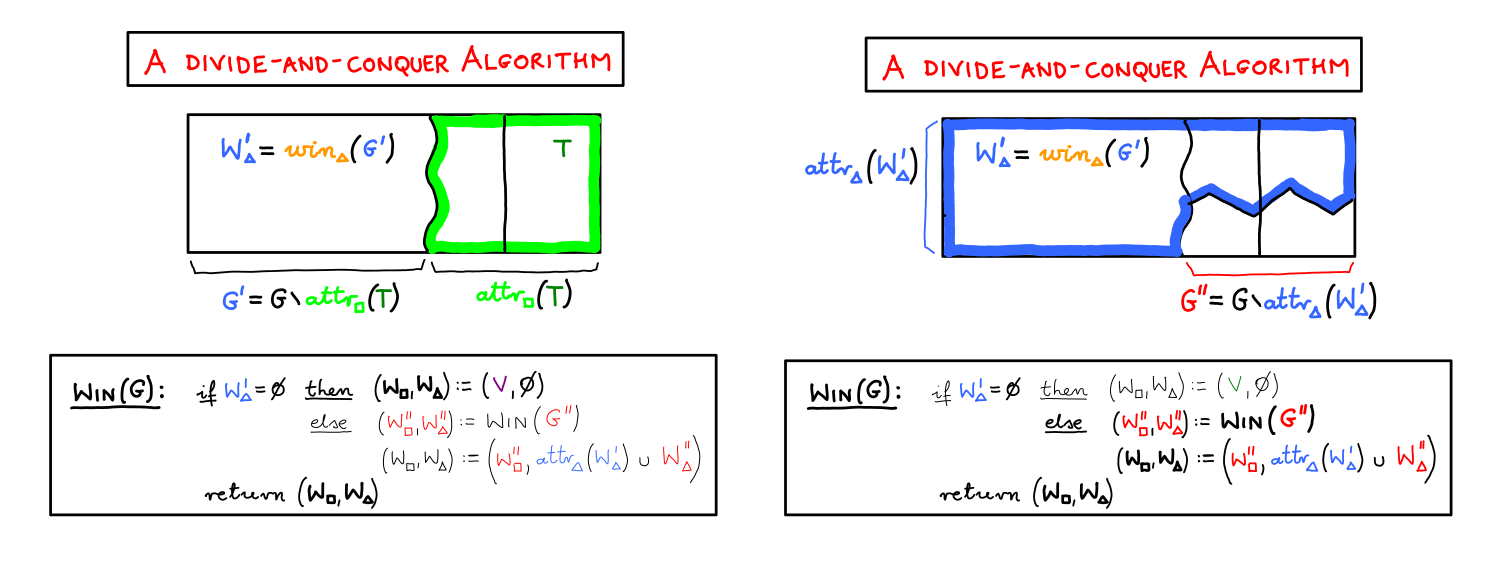
\includegraphics[width=12cm,height=5cm]{buchi.png} \end{center}


\begin{theorem}
B\"uchi games:
\en
% \- The winning regions partition $V$. This is called \emph{determinacy}.
\- Positionally determined (i.e., the positional-winning regions partition $V$).
\- Player $i$ has a positional strategy that is winning from all vertices in $W_i(G)$.
\- Solving can be done in \ptime, i.e., $O(|V|\times |E|)$.
\ne
\end{theorem}

\begin{proof}
	Let $G$ be a repeated-reachability game. 
	
	\begin{itemize}  
	 \item Let $V' = V \setminus \att_0(T)$. 
	 \item If $V' = \emptyset$ then $\WR_0(G) = V$ and $\WR_1(G) = \emptyset$.
	 \item Otherwise, let $V'' = V \setminus \att_1(V')$. 
	\item By recursion solve the game on arena $G''$ to get $\WR_0(G'')$ and $\WR_1(G'')$.
	\item The winning regions in $G$ are: $\WR_0(G'')$ for player $0$, and $\WR_1(G'') \cup \att_1(V')$ for player $1$.
	\end{itemize}
	
	Note that $V''$ is non-empty, and induces a sub-arena (i.e., no dead-ends) $G''$: edge set $(V'' \times V'') \cap E$, 
	target set $T \cap V''$.	The size of $|V''| < |V|$. 
	
		Let $T(n)$ be the maximum number of steps this algorithm takes on arenas with $n$ vertices.
	Then $T(1) = 1$, and $T(n) \leq T(n-1) + O(|E|)$. Thus $T(n) = O(|V| |E|)$.

	
	\paragraph{We claim that $\WR_0(G'') = \WR_0(G)$ and $\WR_1(G'') \cup \att_1(V') = \WR_1(G)$} By squeezing, it is enough to show $\WR_0(G'') \subseteq \WR_0(G) \subseteq \WR_1^c(G) \subseteq \WR_0(G'')$.
% 	$\WR_0(G'') \subseteq \WR_0(G)$ and $\WR_1(G'') \cup \att_1(V') \subseteq \WR_1(G)$. I.e., 
	
	Clearly, $\WR_0(G'') \subseteq \WR_0(G)$. Why? Because $G''$ is a trap for player $1$ in $G$, i.e., being the complement of an attractor, 
	every edge $(v,w) \in E$ (not $E''$!) with $v \in V'' \cap V_1$ has $w \in V''$.
	
	Clearly, $\WR_1(G'') \cup \att_1(V') \subseteq \WR_1(G)$. Why? First, from $v \in \att_1(V')$, \po can ensure that from some point on $T$ 
	is seen only finitely often (attract to $V'$, and then avoid $T$). Second, from $v \in \WR_1(G'')$, \po plays a winning strategy for $G''$. 
	If the play never leaves $G''$ then $T$ is seen finitely often. If the play leaves $G''$ then we are in the first case $v \in \att_1(V')$, 
	and from that point on $v$ visits $T$ finitely often.		
	
\end{proof}


\section{Parity games}

A \emph{colored-arena} is of the form $(A,c)$ where $c:V \to \mathbb{N}$ is the coloring function.
\emph{Parity Objective} = max parity even.

Show that we can define Buchi conditions as parity conditions. Which set of colors suffice? What about co-Buchi? What is the objective if the colors are $\{1,2,3,4\}$?

\begin{center}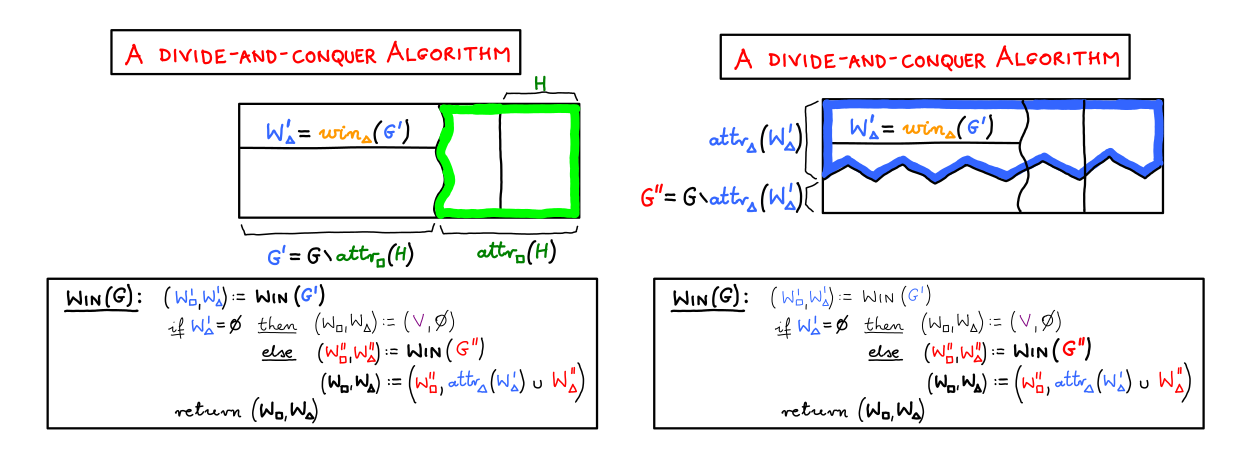
\includegraphics[width=12cm,height=5cm]{parity.png} \end{center}

\begin{theorem}
 Parity games:
\en 
\- Positionally determined (i.e., the positional-winning regions partition $V$).
\- Player $i$ has a positional strategy that is winning from all vertices in $W_i(G)$.
\- Solving can be done in \np and in co-\np, and in time $O(n^{d+O(1)})$.
\ne
\end{theorem}
\begin{proof}
 Induction on $|V|$. 
 
 Let $d$ be highest priority, say even, and let $D = c^{-1}(d)$. 
 
 Let $A = Att_0(D)$.
 
 \begin{enumerate}
  \item If $A = V$ then apply attractor strategy to get to $A$, and from $A$ take any step.
 
  \item If $A \subset V$, then consider the subarena $V \setminus A$. By induction it is uniform positionally determined. 
 Let $W_i$ be the WRs of this subarena.	There are two subcases.
 
 \begin{enumerate} 
 \item $W_1 = \emptyset$, i.e., $W_0 = V \setminus A$. In this case $WR_0 = V$. Indeed, define $\sigma_0$: if in $A$ attract to $d$; if in $D$ do an arb step; if in $V \setminus A$ play given winning strategy in $V \setminus A$.
 
 Take player $\pi$ consistent with $\sigma_0$. Two cases: $\pi$ is in $A$ infinitely often (then it sees $D$ infinitely often); $\pi$ is in $V \setminus A$ from some point on, so this suffix has max parity even. So original play has max parity even.
 
 \item $W_1 \neq \emptyset$. Let $V' = Att_1(W_1)$ (in $G$). 
 
 Then: $V' \subseteq WR_1$, and the following strategy is memoryless: while in $W_1$ play the corresonding ws (note that this is a trap for player $0$, so the play does not leave $W_1$), and while in $V' \setminus W_1$, attract to $W_1$. 
 
 Let $V'' = V \setminus V'$. Since $V''$ is a trap for player $1$, it is a subarena. Solve this recursively to get its winning regions $W''_0$ and $W''_1$. 
 
 Then: $W''_0 \subseteq WR_0$, and the strategy on $W''_0$ is memoryless by induction (and play stays in $W''_0$, so is winning in the original game).
 
 Also: $W''_1 \subseteq WR_1$, and the following strategy is memoryless: use the strategy ``while in $W''_1$ play the corresponding ws``. Note that if a generated play stays in $W''_1$ it is won by player $1$, but if it ever leaves (to the choice of player $0$) it can only leave to $V'$, and thus is also won by player $1$.
 \end{enumerate}
 \end{enumerate}
 \end{proof}

 Computing winning region can be done in time $O(2^n)$; just use the recurrence $T(1) = 1$ and $T(n) \leq 2T(n-1) + O(m)$.
 
 More careful analysis gives $O(n^{d+O(1)})$. Recurrence: $T(n,d) \leq n \times T(n,d-1) + O(n^2)$ and $T(n,1) = O(1)$.

 
 SHOW: solitaire parity games solvable in ptime.
 
 if all nodes belong to player i, find a cycle with largest priority $i mod 2$.
 
 idea: suppose $i,d$ are even. check if there is a path from initial state to a node labeled $d$ and a path from that node to itself. if yes, done.
 if not, remove all nodes labeled $d$ and $d-1$, and repeat.
 
 
% \begin{definition}
% GR(1) ... 
% \end{definition}

% \begin{proof}
% Let $G$ be a repeated-reachability game.
%  Let $Y_0 = T$, $Y_{k+1} = \att^+_0(T \cap Y_k)$. There exists $n$ such that $Y_n = Y_{n+1}$.
%  We claim that $\WR_0(G) = \att_0(Y_n)$.
%  
%  \paragraph{We prove that $Y_n \subseteq \WR_0(G)$}
%  From $\att_0(Y_n) \setminus Y_n$ play a positional strategy that attracts to $Y_n$.
%  From $v \in Y_n = Y_{n+1} = \att^+_0(T \cap Y_n)$, play a positional strategy that attracts to $T \cap Y_n$.
%  Clearly every play $\pi$ consistent with this strategy reaches $T$ infinitely often.
%  
%  \paragraph{We prove that $\WR_0(G) \subseteq Y_n$}
%  By squeezing, it is enough to show that $V \setminus \att_0(Y_n) \subseteq WR_1(G)$. 
%  So, for $V \setminus \att_0(Y_n)$ let $\rank(v)$ be the smallest $i \leq n$ such that $v \not \in Y_i$. 
%  We define a positional strategy such that, from $v$, every play visits $T$ at most $\rank(v)$ times. This is done using the following properties for $v \in V \setminus \att_0(Y_n)$:
%  
%  \begin{enumerate}
%   \item If $v \in V_1 \setminus T$ then there exists $(v,w) \in E$ such that $\rank(w) \leq \rank(v)$.
%   \item If $v \in V_1 \cap T$ then there exists $(v,w) \in E$ such that $\rank(w) < \rank(v)$.
%   \item If $v \in V_0$ then for every $(v,w) \in E$, $\rank(w) \leq \rank(v)$.
%   \item If $v \in V_0 \cap T$ then every $(v,w) \in E$ has $\rank(w) < \rank(v)$.
% \end{enumerate}
% 
% To see (1): suppose otherwise, i.e., every $(v,w) \in E$ has $\rank(w) > \rank(v)$. So $w \in Att^+_0(Y_{\delta(v)})$.
% \end{proof}


% Definitions
% \it
% \- A play $\rho = \rho_0 \rho_1 \dots$ \emph{visits} $T$ if some $\rho_i \in T$.
% \- Positional strategy for player $0$ is a function $\sigma:V_0 \to V$ such 
% that $(v,\sigma(v)) \in E$.
% \- A play $\rho = \rho_0 \rho_1 \dots$ is \emph{consistent} with $\sigma$ if 
% whenever $\rho_i \in V_0$ then $\rho_{i+1} = \sigma(\rho_i)$.
% \- $\sigma$ is \emph{winning} if every play consistent with it reaches $T$. 
% \- Algorithmic problem: Can one decide, given a game $G = (A,T)$ a vertex $v$, 
% if player $0$ has a winning strategy?
% \- Question: In reachability games, if $0$ cannot force a visit to $T$ from 
% $v$, does this mean that $1$ can force the play to avoid $T$?
% \ti
% 
% 
% 
% \subsection{Games with (finite-string) regular objectives}
% Definition, example, example strategy, solving games, reducing to games with reachability objectives, strategy synthesis, determinacy.
% 
% - start with DFA
% 
% Question: what if start with NFA? regular expression?
% 
% 
% \section{Games with quantitative objectives: mpg}
% 
% 
% \section{Multiplayer games and Nash equilibria}
% 


 \section{Games with quantitative objectives}
\paragraph{Outline}
Games with quantitative objectives assign a real number to every play, and one player is trying to maximise this value while the other is trying to minimise it. We will discuss how to solve mean-payoff games.

\begin{center}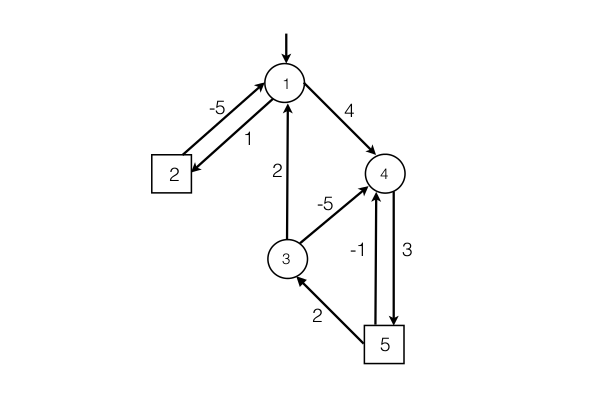
\includegraphics[width=6cm,height=4.6cm]{mpg.png} \end{center}

\emph{edge-colored arena} $(A,w:E \to [-W,+W])$. 

\emph{MP-Objective} is all $\pi = \pi_0 \pi_1 \cdots$ such that:
\[
(\lim_{n \to \infty} \inf avg_n) \geq 0
\]
where $avg_n = \frac{1}{n}\sum_{i=1}^n (w(\pi_{i-1},\pi_{i}))$.

Some calculations: consider play $[12]^\omega$. The sequence of weights is $[1,-5]^\omega$. Thus the 
average for $n$ even is $\frac{-4x}{2x} = -2$, and the average for $n$ odd is $\frac{-4x+1}{2x} \to -2$. 
Thus the mp is $-2$.

consider the play $1[453]^\omega$. The sequence of weights is $4 [3,2,-5]^\omega$. The average for $n \equiv 1 \mod 3$ 
is $4/n$ which tends to $0$. Similarly for the others. So the mp is $0$.

Consider the play $[1453]^\omega$. The sequence of weights is $[4,3,2,2]^\omega$. The average for $n \equiv 0 \mod 4$ is 
$11/4$. Similarly the others tend to $11/4$. so the mp is $11/4 = 2.75$.

\begin{theorem}
 MPG are positionally determined, using uniform strategies, and solving them is in $\np$ and co-$\np$.
\end{theorem}

Proof is postponed till next lecture.

Meanwhile:
\begin{proposition}
 Solving Parity games can be reduced to mean-payoff games in polynomial time.
\end{proposition}
\begin{proof}
 WLOG, colors are in $[d-1]$. Define weight of $(v,w)$ to be $(-1)^i n^i$ where $c(v) = i$ and $n = |V|$. 
 In particular, supposing $d$ is even, the weights are from the set $\{-n^{d-1}, n^{d-2}, ..., -n, 1\}$.
 
 
 It is sufficient to show (*) that for every pair of memoryless strategies, the same strategy wins both games: indeed, 
 suppose pl $i$ has a ws in PG. Then by mem det of PG this can be taken to be a memless strategy. If pl $i$ has no ws in MPG 
 then by memdet pl $1-i$ does, and this can be taken to be memless. By (*) for this pair of memless strategies, 
 the same strategy wins both games. but this is impossible.
 
 To prove (*), fix a pair of memless strategies, and note that a cycle $C$ is formed which governs the winner. 
 Note that $avg(C) \geq 0$ iff $sum(C) \geq 0$. We show that the max col $c$ on $C$ is even iff $sum(C) \geq 0$.
 Let $x$ be weight with largest absolute value. 
 
 Suppose max col on $C$ is even. Then $x > 0$, and so 
 \[sum(C) \geq  x - (n-1)x/n = x/n > 0
 \]
 since there are at most $n-1$ other edges on the cycle, each of whose weight is at most $x/n$.
 The other direction is symmetric.
\end{proof}


\section{First Cycle Games}

% \begin{question}
% Find game that is not positionally determined. Find winning conditions that result in games that are not, in general, positionally determined. 
% Can you solve these games? e.g., occ = V, or generalised reachability.
% \end{question}

We already saw a game that was not positionally determined. Can we characterise those games that are? We introduce FCG. To motivate them notice that if players can win positionally, then fixing positional strategies, the resulting play is a lasso, and who wins (for prefix independent games) depends only on this cycle. 

\begin{definition}
A \emph{Edge-colored arena} is a tuple $(A,\lambda:E \to \mathbb{U})$.

A \emph{cycle property $Y$} is a subset of $\mathbb{U}^*$.

A \emph{first-cycle objective wrt $Y$, written $FC(Y)$} consists of all plays $\pi$ whose first cycle $C_1(\pi)$ is in $Y$. 

A \emph{first-cycle game (FCG)} is a game with a first-cycle objective.

\end{definition}

% e.g., even-length, parity, average is at least k, average/sum is positive.
% 
% \begin{definition}
% %  The set of \emph{cycles} of a play is the output of the procedure that reads the edges of the play onto a stack and removes and output the cycles as they appear.
%  
% \end{definition}

Remark: we transform vertex labeled games into edge labeled games by labeling an edge $(u,v)$ by the label of its source $v$.

Finitise the following objectives: Buchi, Parity, MP. 
\begin{example}
 \it
 \- the cycle should contain an edge from $T$ (i.e., $u \in Y$ iff $u_i \in T$ for some $i$)
 \- the largest priority occuring on the cycle is even (i.e., $u \in Y$ iff $\max_i c(u_i)$ is even)
 \- the average of the weights on the cycle is non-negative (i.e., $u \in Y$ iff $avg(u) \geq 0$).
\ti
\end{example}
% Here are some other useful cycle properties:
% \ti
%  \- the length of the cycle is even.
%  \- the set of vertices on the first cycle should be the set $T$.
%  \- the set of vertices on the first cycle should be a set from $\{T_1, T_2, \cdots, T_k\}$.
%  \ti
% \end{example}


Fact 1. first-cycle games are determined (why?). 

Fact 2. Not necc. positionally determined (use even-length)

Fact 3. Even if positionally determined, not necc. uniform positionally determined (see diagram with property 'ends in 1').

 \begin{center}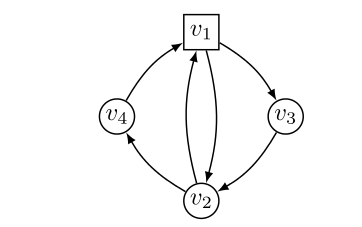
\includegraphics[width=10cm,height=4cm]{fcg-notpositional.png} \end{center}
 \begin{center}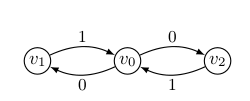
\includegraphics[width=10cm,height=4cm]{fcg-notuniform.png} \end{center}

\begin{definition}
An \emph{edge-path} is a sequence of edges $e_1 e_2 \cdots$ such that $trg(e_i) = src(e_{i+1})$ for all $i$. An edge-path is \emph{simple} if $i \neq j$ implies $trg(e_i) \neq trg(e_j)$.
Extend $\lambda$ to sequences, i.e., $\lambda(s e) = \lambda(s) \lambda(e)$ for $s \in E^*, e \in E$.

%  Let $s = f_1 f_2 \cdots f_m$ be a finite simple edge-path, and $\pi = e_1 e_2 \cdots$ be an edge-path, and if $s$ is non-empty then $last(s) = first(\pi)$, i.e., $s \pi$ is an edge-path.
 
%  Define a process called the \emph{cycles decomposition} of a pair $(s,\pi)$. We describe one step. 
%  The \emph{update} of $(s,\pi)$ is the pair $(s',\pi')$ defined as follows: $\pi' = e_2 e_3 \cdots$; 
%  if $last(e_1)$ does not appear in $s$, then $s' = s \cdot e_1$;  otherwise, suppose $start(f_i) = last(e_1)$, 
%  then $s = f_i f_{i+1} ... f_m e_1$ is a cycle, and define $s' = f_1 \cdots f_{i-1}$.
%  
%  For $\pi$ an infinite edge-path, let $C(\pi)$ be the sequence of cycles produced by repeatedly applying the update starting with $(\epsilon,\pi)$. 
\end{definition} 

\def\src{\textsf{src}}
\def\trg{\textsf{trg}}


The \emph{cycles-decomposition of an edge-path} takes as input
a (usually empty) simple path $s$, which is treated as the initial contents of a stack, and a path $\pi$ (finite or infinite).
At step $j \geq 1$, the edge $\pi_j$ is pushed onto the stack and if, for some $k$, the top $k$ edges on the stack form a cycle, this cycle is output, then popped, and the procedure continues to step $j+1$.

 \begin{center}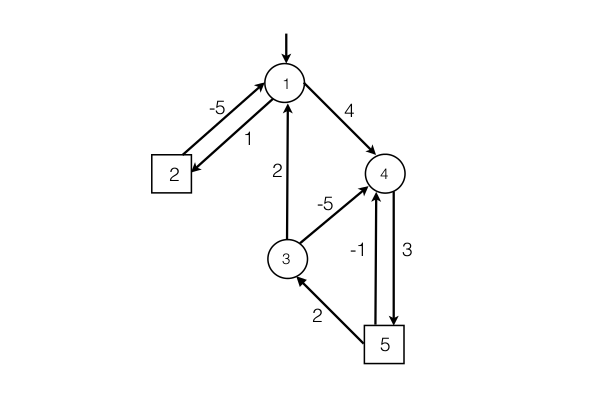
\includegraphics[width=6cm,height=4.6cm]{mpg.png} \end{center}

\begin{example}
What are the sequence of cycles output by the cycles decomposition of 
\[ (1,2)(2,1)(1,2)(2,1)(1,4)[(4,5)(5,3)(3,4)]^\omega\]
\end{example}

\begin{algorithm}[htb]
\caption{Cycles-Decomposition $CD(s,\pi)$}
\label{alg:CD}
\begin{algorithmic}
\Require $s$ is a finite (possibly empty) simple path               \Comment{initial stack content}
\Require $\pi$ is a finite or infinite path $\pi_1 \pi_2 \cdots$    \Comment{the path to decompose}
\Require If $s$ is non-empty then $\trg(s) = \src(\pi)$                \Comment{$s \pi$ must form a path}
\State $ step = 1$
 \While{$ step \leq |\pi|$}								\Comment{Start a step}
\State Append $\pi_{step}$ to $s$						\Comment{Push current edge into stack}
\State Say $s = e_1 e_2 \cdots e_m$
\If{$\exists i: e_i e_{i+1} \cdots e_m$ is a cycle}			\Comment{If stack has a cycle}
\State \textbf{Output} $e_i e_{i+1} \cdots e_m$             \Comment{output the cycle}
\State $s := e_1 \cdots e_{i-1}$ 							\Comment{Pop the cycle from the stack}			
\EndIf
\State $ step :=  step + 1$                                 \Comment{advance to next input edge}
\EndWhile
\end{algorithmic}
\end{algorithm}

\begin{definition}
Let $Y$ be a cycle property. For an infinite path $\pi$, let $first(\pi)$ be the first cycle output by $CD(\epsilon,\pi)$.
The \emph{first-cycle objective based on $Y$, written $FC(Y)$} is the set of plays such $\lambda(first(\pi)) \in Y$.
\end{definition}

Define $N_z(\pi) \in \mathbb{N} \cup \{\infty\}$ to be the index of the first edge that starts with $z$, if one exists.  Define $head_z(\pi)$ to be the prefix of $\pi$ before $N_z(\pi)$, and 
$tail_z(\pi)$ to be the suffix of $\pi$ starting at $N_z(\pi)$. 

Formally, $N_z(\pi):= \infty$ if $z$ does not occur on $\pi$, and otherwise $N_z(\pi) := \min\{j : \src(\pi_j) = z\}$. Also, 
$head_z(\pi) := \pi[1,N_z(\pi)-1]$ and $tail_z(\pi) := \pi[N_z(\pi), |\pi|]$. 
By convention, if $N_z(\pi) = \infty$ then $head_z(\pi) = \pi$ and $tail_z(\pi) = \epsilon$.

We now define a game, that is very similar to the first-cycle game, except that one of the nodes $z$ of the arena is designated as a ``reset'' node... the first time play sees $z$ (if at all), the history is erased:
\begin{definition}
Fix an arena $A$, a vertex $z \in V$, and a cycle property $Y$. Define the objective $FC_z(Y)$ to consist of all plays $\pi$ satisfying the following property: if $head_z(\pi)$ is not a simple path then $first(\pi) \in Y$, and otherwise $first(tail_z(\pi)) \in Y$.
\end{definition}

Playing the game with objective $FC_z(Y)$ is like playing the first-cycle game over $Y$, however, if no cycle is formed before reaching $z$ for the first time, the prefix of the play up to that point is ignored. Thus, in a sense, the game is reset. Also note that if play starts from $z$, then the game reduces to a first-cycle game.


\begin{definition}
Fix $Y$.
An arena is {\em $Y$-resettable} if for every $i \in \{0,1\}$, and every node $z$, we have that
$\WR^i(A,FC_z(Y)) = \WR^i(A,FC(Y))$.
\end{definition}

\begin{theorem}[Resettability implies memoryless determinacy]  \label{EM}
Suppose that every arena $A$ is $Y$-resettable. Then every 
game $(A,FC(Y))$ is memoryless determined.
\end{theorem}

The proof relies on the fact that we may assume that a strategy of $(A,FC_z(Y))$ makes the same move every time it reaches $z$.

\begin{definition}[Forgetful at $z$ from $v$]
Fix an arena $A$, a vertex $v \in V$, a Player $i \in \{0,1\}$, and a vertex $z \in V_i$ belonging to Player $i$. We call a strategy $T$ for Player $i$ {\em forgetful at $z$ from $v$} if there exists $z' \in V$ such that $(z,z') \in E$ and for all $\pi \in plays(T,v)$, and all $n \in \mathbb{N}$, if $\src(\pi_n) = z$ then $\trg(\pi_n) = z'$.
\end{definition}

\begin{lemma}[Forgetful at $z$ from $v$]\label{lem:forgetful at z}
Fix  an arena $A$, a vertex $v \in V$,
a Player $i \in \{0,1\}$, and a vertex $z \in V_i$ belonging to Player $i$.
In the game $(A,FC_z(Y))$, if Player $i$ has a strategy $S$ that is winning from $v$, then Player $i$ has a strategy $T$ that is winning from $v$ and that is forgetful at $z$ from $v$.
\end{lemma}

\begin{proof}[Sketch] 
The second time $z$ appears on a play, the winner is already determined, and so the strategy is free to repeat the first move it made at $z$. On the other hand, the first time $z$ appears on a play, 
the strategy can make the same move regardless of the history of the play before $z$, because the winning condition ignores this prefix.
\end{proof}
% 
% \begin{definition} \label{dfn:resettable}
% For an arena $A$, and a node $v$ in $A$, say that $A$ is {\em $Y$-resettable from $v$} if for every node $z$,
% the same player wins from $v$ in both $(A,FC(Y))$ and $(A,FC_z(Y))$.
% \end{definition}
% 
% 
% First, we show that $Y$-resettability is a sufficient condition for having memoryless strategies.

% \begin{definition}
%  A game $G$ is \emph{memoryless from $v \in V$} if the player that wins from $v$ has a memoryless winning strategy from $v$.
% \end{definition}


\begin{proof}[Sketch of Theorem~\ref{EM}]

% Say that $A$ is \emph{$Y$-resettable from $v$} if for every node $z$, the same player wins from $v$ in both $(A,FC(Y))$ and $(A,FC_z(Y))$.

A node $z \in V$ is a {\em choice node} of an arena $B$, if there are at least two distinct  vertices $v',v'' \in V$ such that $(z,v') \in E^B$ and $(z,v'') \in E^B$.

For each $i \in \{0,1\}$, we induct on the number of choice nodes of player $i$, i.e., the $k$th inductive hypothesis says that in every arena with $k$ choice nodes of player $i$, if player $i$ has a winning strategy from $v$, player $i$ also has a memoryless winning strategy from $v$.

Base case ($k = 0$): this is immediate since there is a single strategy for player $i$, which is memoryless.

Inductive step ($k > 0$). Consider an arena $A$ with $k > 0$ choice nodes for player $i$, and suppose player $i$ has a winning strategy in $(A,FC(Y))$ from $v$.  
Let $z$ be a choice node for Player $i$. 

\it
\- By the resettability assumption applied to $A$, Player $i$ has a winning strategy from $v$ in $(A,FC_z(Y))$.
\- By Lemma~\ref{lem:forgetful at z}, Player $i$ has a strategy $S$ that is winning from $v$ and that is also forgetful at $z$ from $v$. Thus we may form a sub-arena $B$ of $A$ by removing all edges from $z$ that are not taken by $S$. Observe that $S$ is winning from $v$ in $(B,FC_z(Y))$. 
\- Applying the resettability assumption to $B$, Player $i$ has a winning strategy from $v$ in $(B,FC(Y))$.
\- But $B$ has less choice nodes for Player $i$, and thus, by induction, Player $i$ has a memoryless winning strategy from $v$ in $(B,FC(Y))$. 
\ti
This memoryless strategy is also winning from $v$ in $A$ (since we only removed choices of player $i$, which are not used in this memoryless strategy).
\end{proof}



\subsection*{Connection with infinite duration games}

\cbstart
We now define the connection between first-cycle games and games of infinite duration (such as parity games, etc.), namely the concept of $Y$-greedy games. We then prove the Strategy Transfer Theorem, which says, roughly, that for every arena, the winning regions of the First-Cycle Game over $Y$ and a $Y$-greedy game coincide, and that memoryless winning strategies transfer between these two games.
\cbend

\begin{definition}[Greedy]\label{dfn: greedy}
Fix an arena $A$.
The \emph{all-cycle objective based on $Y$, written $AC(Y)$} is the set of plays $\pi$ of $A$ such that the labelling of every cycle output by $CD(\epsilon,\pi)$ is in $Y$.

Say that a {\em game $(A,O)$ is $Y$-greedy} if
\[
AC(Y) \subseteq O \textrm{ and }
AC(\neg Y) \subseteq \neg O.
\]
\end{definition}

% Intuitively, a game $(A,O)$ is $Y$-greedy means that Player $0$ can win the game $(A,O)$
% if he ensures that every cycle in the cycles-decomposition of the play is in $Y$,
% and Player $1$ can win if she ensures that every cycle in the cycles-decomposition of the play is not in $Y$.


The following lemma says that only finitely many edges in a path are pushed but never popped. In particular, at most $|V|-1$ edges:
\begin{lemma}\label{lem:V-1}
For every path $\pi$ in arena $A$ with vertex set $V$, there are at most $|V|-1$ indices $i$ such that $\pi_i$ does not appear in any of the cycles in $cycles(\pi)$.
\end{lemma}

\begin{example} \begin{enumerate}
\item $(A,AC(Y))$ is $Y$-greedy.
\item Every parity game is $Y$-greedy where $Y$ says ``the largest occuring color is even''.
\item Every game with mean-payoff winning condition is $Y$-greedy where $Y$ says ``the average of the cycle is non-negative'' (HW)
\end{enumerate}
\end{example}



We state the Strategy Transfer Theorem:

\begin{theorem}[Strategy Transfer] \label{thm:greedy}
Let $(A,O)$ be a $Y$-greedy game, and let $i \in \{0,1\}$.
\begin{enumerate}
\item $WR^i(A,O) = WR^i(A,FC(Y))$ (so, in particular, $(A,O)$ is determined).
\item For every memoryless strategy $S$ for Player $i$, and vertex $v \in V$:
 $S$ is winning from $v$ in the game $(A,O)$ if and only if $S$ is winning from $v$ in the
    game $(A,FC(Y))$.
\end{enumerate}
\end{theorem}


\def\pumpS{S^{\circlearrowleft}}
\def\pump{\circlearrowleft}

To prove the Strategy Transfer Theorem we need a lemma that states that one can pump a strategy $S$ that is winning for the first-cycle game to get a strategy $\pumpS$ that is winning for the all-cycles game.

The strategy $\pumpS$ says to \textbf{follow $S$ until a cycle is formed, remove that cycle from the history, and continue}. 

Roughly, $\pumpS(u) = stack(u)$ where $stack(u)$ is the stack content of CD after processing path $u$. The fact that every winning strategy in the first-cycle game of $Y$ can be pumped to obtain a winning strategy in a $Y$-greedy game, is why we call such games ``greedy''.

% Recall our notational abuse (Page~\pageref{notational_abuse}) that for a finite path $\rho$, we may write $S(\rho)$ instead of $S(\ver(\rho))$.

\cbstart
First, we need notation to go from edge-paths to node-paths and back: 
\it
\- For simple path $\pi = e_1 e_2 \cdots e_l \in E^*$ write $nodes(\pi)$ for $\src(e_1) \src(e_2) \cdots \src(e_l)\trg(e_l) \in V^*$. 
\- For path $u = v_1 v_2 \cdots v_l \in V^*$ with $l \geq 2$, write $edges(u)$ for $(v_1,v_2) (v_2,v_3) \cdots (v_{l-1},v_l) \in E^+$. 
\ti

Instead of writing these transformations we assume them implicitly.

\begin{definition}[Pumping Strategy]\label{dfn:pumping}
For a finite path $\pi \in E^*$, the stack content at the end of $CD(\epsilon,\pi)$ (Algorithm~\ref{alg:CD}) is denoted $stack(\pi)$. 

Fix an arena $A$,  a Player $i \in \{0,1\}$, and a strategy $S$ for Player $i$. Define the {\em pumping strategy of $S$} be the strategy $\pumpS$ 
on history $u = u_1 \dots u_k$ ending in a node of player $i$, as follows:
\[ 
\pumpS(u) =
	\begin{cases}
	S(u_1) & \mbox{ if } k = 1\\
% 	S(u_k) & \mbox{ if } k > 1, stack(edges(u)) = \epsilon\\
% 	S(nodes(stack(edges(u)))) & \mbox{ otherwise.}
	S(u_k) & \mbox{ if } k > 1, stack(u) = \epsilon\\
	S(stack(u)) & \mbox{ otherwise.}
	\end{cases}
\]
\end{definition}

Note that $\pumpS$ is well-defined since: if $stack(u) \neq \epsilon$ then $stack(u)$ ends with $u_k \in V_i$ and so $stack(\pi)$ is in the domain of $S$. 

\cbend

\begin{lemma}[equal] \label{lem:memless}
If $S$ is memoryless then $\pumpS = S$.
\end{lemma}
\begin{proof}
We need to show that $\pumpS(u) = S(u)$ for all $u$. If $|u| = 1$ then this is immediate by construction. If $stack(u) = \epsilon$ then $\pumpS(u) = S(u_k) = S(u)$ since $S$ is memoryless.
If $stack(u) \neq \epsilon$ then $last(stack(u)) = last(u)$. So $\pumpS(u) = S(stack(u)) = S(u)$ since $S$ is assumed memoryless.
\end{proof}




\begin{lemma}[pumping]\label{lem:pumping}
Fix Player $i \in \{0,1\}$ and let $(A,O)$ be a $Y$-greedy game. If $S$ is a strategy for Player $i$ that is winning from $v$ in $(A,FC(Y))$ then $\pumpS$ is winning from $v$ in $(A,O)$.
\end{lemma}

\begin{proof}
The strategy $\pumpS$ says to follow $S$, and when a cycle is popped by $CD$, remove that cycle from the history and continue. Thus, for every cycle $C$ that is popped, let $l$ be the time at which the first edge of $C$ is being pushed, and note that the stack up to time $l$ followed by $C$ is a path consistent with $S$ whose first cycle is $C$.

Thus if $S$ is a strategy of player $0$ that is winning from $v$ in the game $(A,FC(Y))$ then for every play $\pi \in plays(\pumpS,v)$, every cycle in $cycles(\pi)$ is in $Y$. By definition of $Y$-greedy, this means that $\pumpS$ is winning from $v$ in the game $(A,O)$. The case of player $1$ is symmetric.
\end{proof}


\begin{proof}[Proof of Strategy Transfer Theorem]
Let $Y$ be a cycle property and $A$ an arena.  Suppose that $(A,O)$ is $Y$-greedy.
We begin by proving the first item. Use Lemma~\ref{lem:pumping}[pumping] to get that for $i \in \{0,1\}$,
\[
\WR^i(A,FC(Y)) \subseteq \WR^i(A,O).
\]

Since first-cycle games are determined, the winning regions $\WR^0(A,FC(Y))$ and $\WR^1(A,FC(Y))$ partition $V$. Thus, since $\WR^0(A,O)$ and $\WR^1(A,O)$ are disjoint, the containments above are equalities, as
required for item $1$.

We prove the second item. Suppose $S$ is a memoryless strategy for player $0$ and recall that $S = \pumpS$ (by Lemma~\ref{lem:memless}[memless]).

\begin{itemize}
 \item Suppose $S$ is winning from $v$ in the game $(A,FC(Y))$. Then it is winning from $v$ in the game $(A,O)$ (By Lemma~\ref{lem:pumping}).

\item Suppose $S$ is not winning from $v$ in the game $(A,FC(Y))$. Since $S$ is memoryless, plays of $A$ consistent with $S$ are exactly infinite paths in the induced sub-arena $A^{||S}$.
Hence, there is a path $\pi$ in the induced solitaire arena $A^{||S}$ for which the first cycle, say $C$, satisfies $\neg Y$. Define the infinite path $\pi'$ which pumps this cycle forever. 
Being a path in $A^{||S}$, it is a play of $A$ consistent with $S$. Moreover, $\pi'$ has the property that every cycle in its cycles-decomposition (i.e., $C$) satisfies $\neg Y$. 
Since $(A,O)$ is $Y$-greedy, $S$ is not winning from $v$ in the game $(A,O)$.
\end{itemize}
The case that $S$ is a strategy for player $1$ is symmetric.
\end{proof}

Putting together we get: 
\begin{theorem} 
If every arena is $Y$-resettable then every $Y$-greedy game is memoryless determined.
\end{theorem}

\subsection*{Recipe for positional determinacy}
% \begin{center}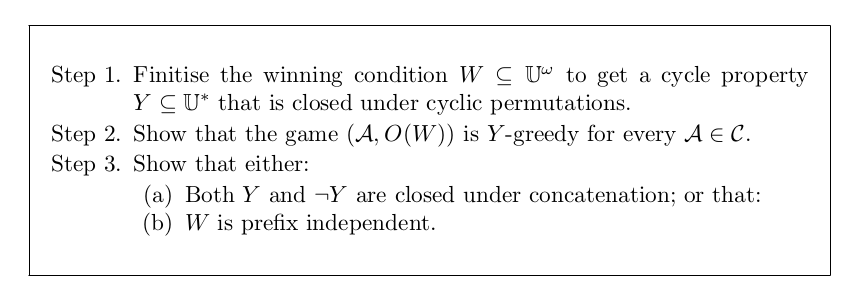
\includegraphics[width=10cm,height=4cm]{fcg.png} \end{center}

\begin{question} 
How to check if every arena is $Y$-resettable? 
\end{question}

\begin{definition}
Fix an arena $A$.
 Let $TAC(Y)$ consist of all plays $\pi$ of $A$ such that some suffix of $\pi$ is in $AC(Y)$.
 An arena $A$ is \emph{$Y$-unambiguous} if there is no play of $A$ that is in $TAC(Y) \cap TAC(\neg Y)$.
\end{definition}

\begin{example}
 If $A$ is $Y$-unambigous then $(A,TAC(Y))$ is $Y$-greedy. Why? clearly $AC(Y) \subseteq TAC(Y)$.
 Also $AC(\neg Y) \subseteq TAC(\neg Y) \subseteq \neg TAC(Y)$ by assumption.
\end{example}

\begin{theorem}[unambigous implies resettable] \label{thm:greedy2}
Every arena that is $Y$-unambiguous is also $Y$-resettable.
\end{theorem}


\begin{proof}
First, if $A$ is $Y$-unambigous then $(A,TAC(Y))$ is $Y$-greedy (above). Thus by Theorem~\ref{thm:greedy} the winning regions of $(A,FC(Y))$ and $(A,TAC(Y))$ coincide.

Second, we now show that the winning regions of $(A,FC_z(Y))$ and $(A,TAC(Y))$ coincide. As usual, it is sufficient to show containment, i.e., 
$WR^i(A,FC_z(Y)) \subseteq WR^i(A,TAC(Y))$ for $i = 0,1$. 

So, suppose player $i$ has a winning strategy $S$ from $v$ in $(A,FC_z(Y))$. 

\textbf{It is sufficient to define a strategy $T$ for player $i$ such that every play consistent with $T$ is in $TAC(Z)$ where $Z = Y$ if $i = 0$ and $Z = \neg Y$ if $i=1$} (why? if $i = 0$ then this is what we want. 
if $i = 1$ then every play consistent with $T$ is in $TAC(\neg Y) \subseteq \neg TAC(Y)$, as required).

There are two cases:
\begin{enumerate}
 \item there is no simple path consistent with $S$ that ends in $z$. Thus $S$ is winning for $FC(Z)$, so $T = \pumpS$ is winning for $AC(Z)$ and thus for $TAC(Z)$.
 \item o/w let $h$ be a simple path consistent with $S$ ending in $z$. Define 
\[
T(u) :=
\begin{cases}
	\pumpS(u) & \mbox{if $z$ does not appear on $u$,}\\
	(S_z)^\pump(tail_z(u)) & \mbox{otherwise.}\\
\end{cases}
\]
where 
$S_z(u) = S(hu)$ if $u$ starts in $z$ (and, otherwise arbitrarily).
 \end{enumerate}
In words, $T$ behaves like the pumping strategy $\pumpS$. Once (and if) $z$ is reached, $T$ erases all its memory and switches to $(S_z)^\pump$ (which itself is winning from $z$ in the FCG). 
Note that $T$ is winning $TAC(Z)$: if $z$ never appears then every cycle is in $Z$; if $z$ does appear, then starting at that point in time, every cycle is in $Z$.
\end{proof}

\begin{question}
Ok, so how to check if $A$ is $Y$-unambigous?
\end{question}

\begin{definition}
 A \emph{winning condition} is a set $W \subseteq \mathbb{U}^\omega$. On an edge-coloured arena $(A,\lambda:E \to \mathbb{U})$ it determines an objective, i.e., $O(W)$ consisting of all 
 plays $\pi$ in $A$ such that $\lambda(\pi) \in W$.
\end{definition}

\begin{example}
 \begin{enumerate}
\item The parity winning condition over $\mathbb{U} = [N]$ consists of all sequences $\alpha \in [N]^\omega$ such that $max inf(\alpha)$ is even.
\item The mean-payoff winning condition over $\mathbb{U} = [-N,N]$ consists of all sequences $\alpha$ such that $\lim_n \inf avg_n(\alpha) \geq 0$.
 \end{enumerate}
 
\end{example}


\begin{lemma}
% Suppose both $Obj$ and $\neg Obj$ are prefix-independent. Let $Y$ be a cycle-property such that every game $(A,Obj)$ is Y-greedy.
% Then every game $(A,Obj)$ is memless determined.
Suppose $W$ and $\neg W$ are prefix-independent, and consider an arena $A$ and a cycle property $Y$. If $(A,O(W))$ is a $Y$-greedy game then $A$ is $Y$-unambiguous.
\end{lemma}

\begin{proof}
Suppose not. Take a play $\pi$ of some arena such that some suffix $\pi' \in AC(Y) \subseteq O(W)$ and some suffix $\pi'' \in AC(\neg Y) \subseteq \neg O(W)$. But one of these is a suffix of the other, say $\pi'$ is a suffix of $\pi''$ (the other case is symmetric). Then $\lambda(\pi') \in W$ is a suffix of $\lambda(\pi'') \not \in W$. 
Contradiction.
\end{proof}

But prefix-independence is typically easy to check! 

\begin{framed}
To conclude that every game with winning condition $W$ is memless determined:
\begin{enumerate}
\item Check that $W$ and $\neg W$ are prefix independent.

\item Finitise the winning condition $W$ to get a cycle property $Y$.

\item Show that every game $(A,O(W))$ is $Y$-greedy.
\end{enumerate}
\end{framed}

\begin{example}
Apply the recipe to B\"uchi, parity-, mean-payoff winning conditions.
e.g., Let $W$ be the buchi condition. it and its complement are prefix-independent.
\end{example}
 


\subsection*{What if the winning-condition is not prefix independent?}

\begin{enumerate}
\item Say that $Y$ is {\em closed under cyclic permutations} if $a b \in Y$ implies
    $ba \in Y$, for all $a \in \mathbb{U}, b \in \mathbb{U}^*$.
\item Say that $Y$ is {\em closed under concatenation} if $a \in Y$ and $b \in Y$
    imply that $ab \in Y$, for all $a,b \in \mathbb{U}^*$.
\end{enumerate}


\begin{theorem} \label{thm: easy}
Let $Y$ be a cycle property. If $Y$ is closed under cyclic permutations, and both $Y$ and $\neg Y$ are closed under concatenation, then every arena is $Y$-unambigous (and therefore $Y$-resettable).
\end{theorem}


\begin{framed}
To conclude that $(A,O(W))$ is uniform memless determined:
\begin{enumerate}

\item Finitise the winning condition $W$ to get a cycle property $Y$.

\item Check that $Y$ is closed under cyclic permutations and both $Y$ and $\neg Y$ are closed under concatenation.

\item Check that $(A,O(W))$ is $Y$-greedy.
\end{enumerate}
\end{framed}

We conclude with a more sophisticated use of the recipe, applied to the initial credit problem of energy games. 

\begin{definition} 
The \emph{Energy winning-condition with initial credit $r$}, written $W_r \subseteq \mathbb{Z}^*$, consists of all sequences $\alpha$ such that $r + \sum_{1 \leq i \leq n} \alpha_i \geq 0$ for all $n$.
\end{definition}

\begin{theorem} 
Either there is an initial credit with which Player $0$ (the ``energy'' player) wins, or for every initial credit Player $1$ wins. In both cases, we show that the winner can use a memoryless strategy. 
\end{theorem}

\begin{proof}
Finitise ``energy'' as $Y \subset \mathbb{Z}^*$ which says that the sum of the numbers is non-negative. This property is clearly closed under cyclic permutations and concatentation, and its complement (the sum is negative) is also clearly closed under concatenation. Also $(A, AC(Y))$ is $Y$-greedy, and thus memoryless determined. 

Claim: if $\sigma$ is a winning strategy for player $0$ in $(A,AC(Y))$ then $\sigma$ is a winning strategy in the energy game on $A$ for some initial credit $r$.

Indeed, let $r = -t (|V|-1)$, where $t$ is the minimum amongst the negative weights of the arena. Let $\pi$ be consistent with $\sigma$, and consider some prefix $\pi'$ of it. 
By Lemma~\ref{lem:V-1}, at most $|V|-1$ edges are not on $cycles(\pi')$, and thus the energy level at the end of $\pi'$ is at least the initial credit plus $t(|V|-1)$. Hence, an initial credit of $r$ suffices for $\pi$ to be winning for Player $0$ also in the energy game. 

Claim: if $\sigma$ is a winning strategy for player $1$ in $(A,AC(Y))$ then $\sigma$ is a winning strategy in the energy game on $A$ for all initial credits.

Indeed, observe that a winning strategy for player 1 in $(A, AC(Y))$ is also winning $(A,FC(Y))$; and thus by pumping is also winning in $(A,EC(Y))$ where $EC(Y)$, the objective for player $0$, says that some cycle should be in $Y$. Thus every play consistent with this strategy has all cycles not in $Y$, and thus in the energy game the energy along the play tends to $-\infty$, and so for every initial credit player $1$ wins. 
\end{proof}





% \subsection*{What about uniformity?}
% 
% [ROUGH]
% 
% 
% We also have a full characterisation in the paper.
% \begin{enumerate}
% \item Say that $Y$ is {\em closed under cyclic permutations} if $a b \in Y$ implies
%     $ba \in Y$, for all $a \in \mathbb{U}, b \in \mathbb{U}^*$.
% \item Say that $Y$ is {\em closed under concatenation} if $a \in Y$ and $b \in Y$
%     imply that $ab \in Y$, for all $a,b \in \mathbb{U}^*$.
% \end{enumerate}
% 
% \begin{theorem}[Memoryless Determinacy  Characterisation of FCGs]\label{thm: memdet all FCG}
% The following are equivalent for every cycle property $Y$:
% \begin{enumerate}
% \item $Y$ is closed under cyclic permutations, and every arena $A$ is $Y$-resettable.
% \item Every game with objective $FC(Y)$ is uniform memoryless determined.
% \end{enumerate}
% \end{theorem}
% 
% \begin{theorem}
% If $Y$ is closed under cyclic permutations then every Y-greedy game that is memoryless determined is also uniform memoryless determined.
% \end{theorem}
% 
% \begin{proof}
%  Enough to show that if $(A,FC(Y))$ memoryless determined implies it is uniform memoryless determined (then use strategy transfer theorem).
% %  Let $S_v$ be a memless strategy winning from $v \in WR_i$. The idea is to define a memoryless strategy $S$ for Player $i$ that is winning from every node $v \in W_i$ by considering the nodes of $W_i$ (in some arbitrary order), and if $v$ is the next node in $W_i$ for which $S(v)$ is not yet defined, then define $S(w) := S_v(w)$ for all $w \in Reach(S_v,v)$ that have not yet been defined. Thus, $S$ is memoryless by construction. The main work is to show that it is winning; in particular, we use the fact that if $Y$ is closed under cyclic permutations and if $S$ is winning from $v$ then $S$ is winning from every node reached from $v$.
% \end{proof}
% 

\section{Games with multiple players}
\paragraph{Outline} 
Games with multiple players require different types of solutions. We will define Nash equilibria on games on graphs, and show how to decide their existence (and compute an equilibrium, if it exists) for certain objectives that we have already encountered.

\section{Different approaches to solving games}

\en
\- PDL satisfiability (Racer, FaCT, Pellet)

\- simulation based techniques

\- safety games, GR(1), ATL

\- Directed search (Stroeder and Pagnucco 09)

\- Planning

\- Antichain

\- Incremental

\- DES

\- parity games: progress measures, rank-based, zielonka

\ne

Reflections: 1 or 2 pars email to me or to florian on reflections on the course: what worked well for you, what didn't, level of interactive, good pace, enjoyable to come to class, connected to other material you learned, learn more than the syllabus e.g., how to formalise intuitions, etc.

\end{document}

